\documentclass[11pt,a4paper]{article}

% ---------------------------------------------------------------------------
%  SupplyForge -- capacity factors & data-source interactions
%  Author: Simon Brigode <simon.brigode@ehess.fr>
% ---------------------------------------------------------------------------
\usepackage[utf8]{inputenc}
\usepackage[T1]{fontenc}
\usepackage{lmodern}
\usepackage[a4paper,margin=2.4cm]{geometry}
\usepackage{amsmath}
\usepackage{booktabs}
\usepackage{array}
\usepackage{xcolor}
\usepackage{caption}
\usepackage{enumitem}
\usepackage{fancyhdr}
\usepackage{listings}
\usepackage{tikz}
\usetikzlibrary{positioning,fit,backgrounds,arrows.meta}
\usepackage[hidelinks,colorlinks=true,linkcolor=blue!50!black,urlcolor=blue!50!black]{hyperref}

\pagestyle{fancy}\fancyhf{}
\lhead{\small SupplyForge --- capacity factors \& data-source interactions}
\rhead{\small\thepage}
\renewcommand{\headrulewidth}{0.4pt}

\definecolor{codebg}{gray}{0.95}
\lstset{basicstyle=\ttfamily\small, backgroundcolor=\color{codebg}, frame=single, framerule=0pt,
  breaklines=true, columns=fullflexible, keepspaces=true, xleftmargin=6pt, xrightmargin=6pt,
  aboveskip=8pt, belowskip=8pt}

\tikzset{
  src/.style ={rectangle, rounded corners, draw=blue!55, fill=blue!8, align=center, inner sep=3pt,
               minimum height=7mm, text width=24mm, font=\scriptsize},
  sup/.style ={rectangle, rounded corners, draw=red!60, fill=red!8, align=center, inner sep=3pt,
               minimum height=8mm, text width=32mm, font=\footnotesize},
  dem/.style ={rectangle, rounded corners, draw=teal!70!black, fill=teal!10, align=center, inner sep=3pt,
               minimum height=8mm, text width=32mm, font=\footnotesize},
  mod/.style ={rectangle, rounded corners, draw=violet!65, fill=violet!10, align=center, inner sep=3pt,
               minimum height=8mm, text width=26mm, font=\footnotesize},
  ext/.style ={rectangle, rounded corners, draw=black!45, fill=black!4, align=center, inner sep=3pt,
               minimum height=7mm, text width=24mm, font=\scriptsize, densely dashed},
  flow/.style={-{Latex[length=2mm]}, draw=black!55, thick},
}

\title{\textbf{SupplyForge --- capacity factors \& data-source interactions}\\[2pt]
\large How the load factors are built from each dataset, and how the packages fit together}
\author{Simon Brigode \quad\textendash\quad \texttt{simon.brigode@ehess.fr}}
\date{11 June 2026}

\begin{document}
\maketitle
\thispagestyle{fancy}

\begin{abstract}\noindent
A capacity factor (\emph{facteur de charge}, generation side) is the hourly ratio, in $[0,1]$, of a
technology's output to its nameplate capacity --- the availability signal that drives wind, solar and
run-of-river in the optimisation. SupplyForge can build it from four data sources, each with a different
method but a single shared output schema. This note explains that construction source by source, the
reservoir-inflow reconstruction, and the source-selection machinery; then the demand-side mirror --- how
DemandForge constructs the load curve and where the \emph{load factor} (average over peak load) comes
from; and finally how the SupplyForge (supply) and DemandForge (demand) packages fetch data and interact.
\end{abstract}

\tableofcontents
\bigskip

% ===========================================================================
\section{One output, four sources}
Every source emits the \emph{same} canonical file --- \texttt{results/capacity\_factors/capacity\_factors\_\{country\}\_\{year\}.parquet}
--- with columns \texttt{hour}, \texttt{plant\_type}, \texttt{WS} (weather/climate-year tag),
\texttt{capacity\_factor}. Because the schema is fixed, the model builder
(\texttt{create\_pommes\_craft\_model} / \texttt{grid\_model}) never changes when the source does; it just
reads the file and injects \texttt{capacity\_factor} as a technology's hourly \texttt{availability}. The
four sources (Table~\ref{tab:cf}) differ only in \emph{how} the number is produced.

\begin{table}[ht]\centering\caption{Capacity-factor construction by source.}\label{tab:cf}\small
\begin{tabular}{@{}p{2.1cm}p{4.3cm}p{4.6cm}p{3.4cm}@{}}
\toprule
\textbf{Source} & \textbf{What it is} & \textbf{How CF is built} & \textbf{Status / note} \\
\midrule
\textbf{ENTSO-E} & observed generation + installed capacity (a real historical year) &
  \emph{measured}: $\mathrm{CF}=\text{generation}/\text{installed capacity}$, hourly &
  default; may exceed 1 on data noise (not clipped) \\
\textbf{ERAA 2024} & the ERAA prospective dashboard CFs & already a CF: extract + reshape; 35 weather
  scenarios (WS1--WS35), horizon years &
  prospective; one file per horizon year \\
\textbf{PECD 4.2} & CDS climate product; CF at bidding-zone level &
  \emph{spatial aggregation}: capacity-weighted zone$\to$country (Eq.~\ref{eq:cfnat}) &
  the default for the regional/climate models; clipped to $[0,1]$ \\
\textbf{ERA5 (raw)} & raw ERA5 climate fields &
  \texttt{atlite} conversion + Global-Wind-Atlas bias correction &
  Phase 2 --- not yet wired (\texttt{NotImplementedError}) \\
\bottomrule
\end{tabular}
\end{table}

% ===========================================================================
\section{Construction, source by source}

\subsection{ENTSO-E --- measured (the default)}
For each intermittent plant type $p$ (Solar, Wind Onshore, Wind Offshore, Hydro Run-of-river) and hour
$t$:
\begin{equation}
\mathrm{CF}_{p,t}=\frac{G_{p,t}}{C^{\text{inst}}_{p}}\quad(\text{else }0\text{ if }C^{\text{inst}}_p=0),
\label{eq:cfentsoe}
\end{equation}
with $G$ the ENTSO-E actual generation and $C^{\text{inst}}$ the nationally-aggregated installed
capacity. Inputs: \texttt{generation\_*} + \texttt{installed\_capacities\_*}; the series is resampled to
hourly UTC. \emph{Dispatchable} plants instead get an \textbf{availability} series from outage events,
\begin{equation}
a_{p,t}=1-\frac{U_{p,t}}{C^{\text{inst}}_p},\qquad U_e=\text{nominal power}_e-\text{available}_e,
\label{eq:avail}
\end{equation}
($U_{p,t}$ = sum of overlapping outages), written to \texttt{results/availability/}. This path reflects
what the \emph{actual} fleet did in a real weather + outage year.

\subsection{ERAA 2024 --- prospective scenarios}
The ERAA dashboard already publishes capacity factors, so SupplyForge only \emph{extracts and reshapes}
them: it reads the staged ERAA CSVs (skipping the metadata header), unpivots the 35 weather-scenario
columns into a long \texttt{(hour, WS, capacity\_factor)} frame, labels the technology, and averages if a
technology has multiple files. The \texttt{WS} column (\texttt{WS1}\dots\texttt{WS35}) is the climate-year
axis; horizon years are 2026/28/30/35. No division is needed --- it is already a CF.

\subsection{PECD 4.2 --- capacity-weighted zonal aggregation}
PECD ships CF directly for solar (\texttt{SPV}), onshore wind (\texttt{WON}) and offshore wind
(\texttt{WOF}), but at the \emph{bidding-zone} level. The construction is therefore \textbf{spatial
aggregation} to the country: the national CF is the installed-capacity-weighted average over the
country's zones $z$,
\begin{equation}
\mathrm{CF}_{\text{nat}}(t)=\frac{\sum_z \mathrm{CF}_z(t)\,C_z}{\sum_z C_z}.
\label{eq:cfnat}
\end{equation}
Weights $C_z$ come from a configured per-zone capacity table (config dict $\to$ CSV $\to$ equal-weight
fallback with a loud warning). \textbf{Run-of-river} is the exception: PECD gives \emph{weekly}
generation energy (\texttt{HRO}+\texttt{HPO}), so the CF is reconstructed as
\begin{equation}
\mathrm{CF}_{\text{RoR}}(w)=\frac{\text{HRO}_w+\text{HPO}_w}{C^{\text{inst}}_{\text{RoR}}\times 168\,\text{h}},
\label{eq:cfror}
\end{equation}
then interpolated weekly$\to$hourly (the sub-weekly variability is lost --- flagged). All series are
leap-trimmed (drop Feb~29 $\Rightarrow$ exactly 8760~h) and clipped to $[0,1]$.

\subsection{ERA5 (raw) --- atlite, Phase 2}
The raw-ERA5 engine would build an \texttt{atlite} cutout from ERA5 climate fields, apply turbine
power-curves / a PV model, aggregate grid cells to the country with land-use masks, and correct the wind
bias against the Global Wind Atlas. It emits the same canonical schema, but is not yet production-wired
(the dispatcher raises \texttt{NotImplementedError}).

% ===========================================================================
\section{Reservoir hydro inflow --- two methods}
The reservoir is modelled as a storage fed by a must-run \emph{inflow} signal. The inflow is built two
ways and written to \texttt{results/inflow/} (\texttt{inflow\_MW}, \texttt{timestamp}):
\begin{itemize}[nosep]
  \item \textbf{ENTSO-E water balance} --- weekly inflow = weekly generation + weekly storage change,
        $I_w = G_w + \Delta S_w$, interpolated weekly$\to$hourly, clipped $\ge 0$, divided by 168 to get
        MW. It mixes natural inflow with dispatch decisions.
  \item \textbf{PECD \texttt{HRI}} --- a \emph{natural}-inflow reconstruction (a Random-Forest model of
        weekly temperature + precipitation), summed across the country's zones, interpolated
        weekly$\to$hourly. More physical, since it is not contaminated by dispatch.
\end{itemize}
Downstream the inflow is \emph{shape-normalised} ($\text{availability}=\text{inflow}/\max\text{inflow}$),
so only the temporal \emph{profile} matters --- the absolute scale cancels.

% ===========================================================================
\section{Source selection \& orchestration}
Two \textbf{orthogonal} config switches (in \texttt{sources.py}) choose the source, independently for
renewables and for hydro:
\begin{lstlisting}
res_source:   entsoe | era5 | pecd      # wind & solar capacity factors
hydro_source: auto   | entsoe | pecd    # reservoir inflow + run-of-river
#   auto -> follows res_source where it can supply hydro (pecd->pecd), else entsoe
#           (in particular era5 -> entsoe, since raw ERA5 cannot produce hydro inflow)
\end{lstlisting}
A thin dispatcher routes \texttt{calculate\_capacity\_factors} / \texttt{calculate\_hydro\_inflow} to the
matching processor but writes the \emph{same} canonical output path --- so \texttt{rule all}, the GCS
upload, and the model builder are untouched. The pure \texttt{entsoe}+\texttt{entsoe} combination
delegates to the original code \emph{byte-for-byte} (a hard backward-compatibility rule); any other
combination composes wind/solar from \texttt{res\_source} with RoR from \texttt{ror\_source} into the
canonical schema. Every processor is \emph{fail-soft}: a missing input yields a valid empty file + a
warning, never a crashed DAG.

% ===========================================================================
\section{The demand side: load curves \& the load factor}
\label{sec:loadfactor}
In French, \emph{facteur de charge} covers two distinct English objects. The \textbf{capacity factor}
(\S2) is a \emph{generation}-side property: output over nameplate capacity. The \textbf{load factor} is
the \emph{demand}-side mirror: for a load curve $L(t)$ over a period,
\begin{equation}
\mathrm{LF}=\frac{\bar L}{L_{\max}}
\qquad\text{(average load over peak load, in } (0,1]\text{)},
\label{eq:lf}
\end{equation}
a measure of how \emph{flat} the demand is --- $\mathrm{LF}=1$ would be perfectly flat; a peaky,
heating-driven curve (e.g.\ France in winter) has a lower LF. It is not fetched from any dataset: it is a
\emph{property of the load curve that DemandForge constructs}, and that construction is itself a
per-dataset pipeline:
\begin{enumerate}[nosep]
  \item \textbf{ENTSO-E load} --- the observed hourly national load $L(t)$ for a reference year.
  \item \textbf{ERA5 $\times$ GHSL} --- the \emph{population-weighted} temperature
        $T_{\mathrm{pop}}(t)=\sum_c \mathrm{pop}_c\,T_c(t)\big/\sum_c \mathrm{pop}_c$ (ERA5 2\,m
        temperature on the grid cells where people actually live --- the temperature the load responds
        to, not the area average).
  \item \textbf{Thermosensitivity regression} --- per hour-of-day, linear regressions of load against
        temperature below a winter threshold $T_w$ and above a summer threshold $T_s$ (thresholds chosen
        by maximising the combined $R^2$), giving heating and cooling slopes in MW/$^\circ$C.
  \item \textbf{Decomposition} --- the load is split into additive components,
        \begin{equation}
        L(t)=B(t)\;+\;\beta_w\,\bigl(T_w-T_{\mathrm{pop}}(t)\bigr)^{+}\;+\;
        \beta_s\,\bigl(T_{\mathrm{pop}}(t)-T_s\bigr)^{+}\;+\;\mathrm{EV}(t),
        \label{eq:decomp}
        \end{equation}
        i.e.\ baseload $+$ winter-thermosensitive (heating) $+$ summer-thermosensitive (cooling) $+$ the
        ERAA EV charging profile (day-of-week aligned). Stored as the
        \texttt{combined\_load\_*.parquet} reference file.
  \item \textbf{Projection} (\texttt{project\_load\_curve}) --- each component is scaled
        \emph{independently} to its target-year energy (growth rate or absolute target) and re-summed.
\end{enumerate}
The load factor then \emph{emerges} from the component mix --- which is exactly why the decomposition
matters: growing the thermosensitive share makes the curve peakier ($\mathrm{LF}\downarrow$), heat-pump
electrification reshapes winters, and EV charging adds its own profile. In the SupplyForge models the
distinction is live: a node given a flat \texttt{demand\_TWh} has $\mathrm{LF}=1$ (the simplification
used in the EU greenfield demonstrator), whereas a node given a DemandForge \texttt{demand\_profile}
carries the realistic load factor (the FR--BE regional model). Adequacy-relevant results (peaking
capacity, storage value, load shedding) are sensitive to this choice.

% ===========================================================================
\section{Packages \& how they interact}
SupplyForge (supply) and DemandForge (demand) are \textbf{sibling, decoupled} packages --- neither imports
the other. Each fetches its own raw data, harmonises it, and emits inputs for the same
\texttt{pommes\_craft} / POMMES optimisation, where supply technologies and demand series finally meet
(Figure~\ref{fig:pkg}). They share several upstream sources (ERA5, ERAA, GHSL/GISCO geometry) and all the
conventions (per-\{country,year\} files, Parquet, GCS caching, the \texttt{pommes\_craft} library).

\begin{figure}[ht]\centering
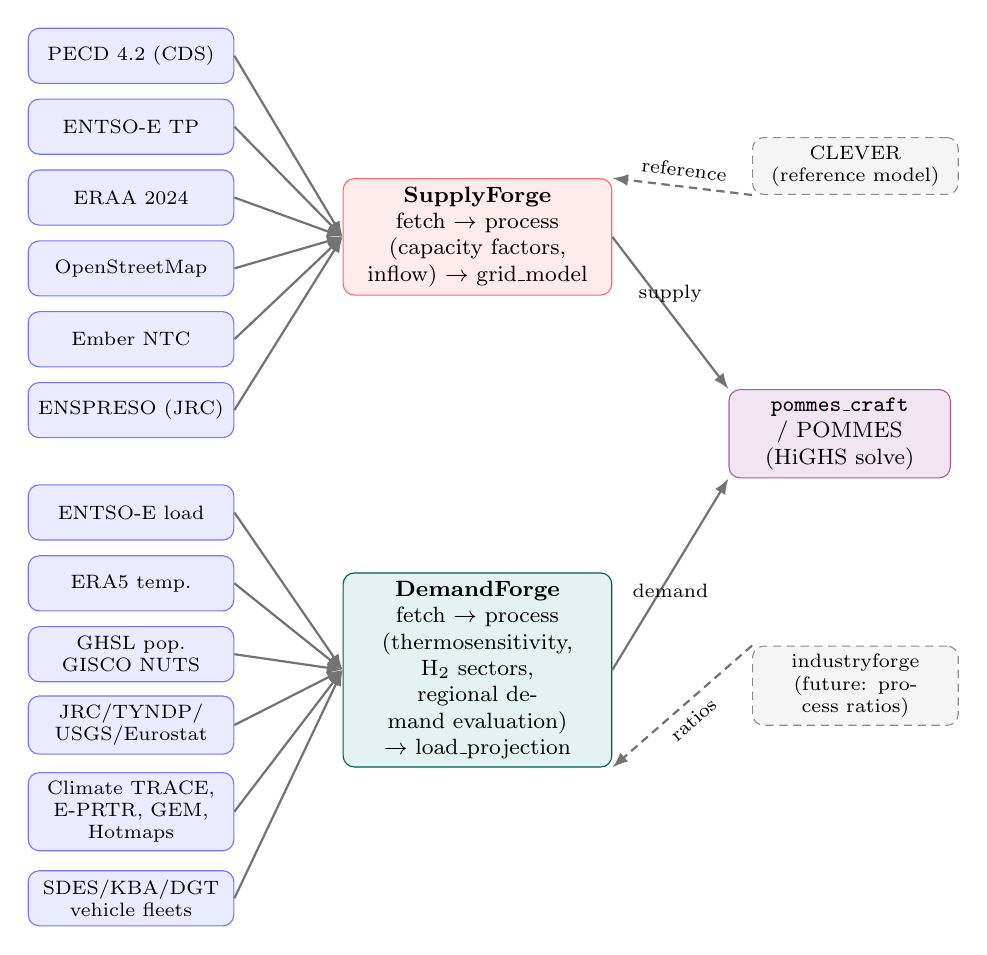
\begin{tikzpicture}
% --- supplyforge sources ---
\node[src] (pecd)  at (0,4.6) {PECD 4.2 (CDS)};
\node[src] (entso) at (0,3.7) {ENTSO-E TP};
\node[src] (eraa)  at (0,2.8) {ERAA 2024};
\node[src] (osm)   at (0,1.9) {OpenStreetMap};
\node[src] (ember) at (0,1.0) {Ember NTC};
\node[src] (ensp)  at (0,0.1) {ENSPRESO (JRC)};
% --- demandforge sources ---
\node[src] (load)  at (0,-1.2) {ENTSO-E load};
\node[src] (era5)  at (0,-2.1) {ERA5 temp.};
\node[src] (ghsl)  at (0,-3.0) {GHSL pop.\\GISCO NUTS};
\node[src] (ind)   at (0,-3.9) {JRC/TYNDP/\\USGS/Eurostat};
\node[src] (fac)   at (0,-5.0) {Climate TRACE,\\E-PRTR, GEM,\\Hotmaps};
\node[src] (fleet) at (0,-6.1) {SDES/KBA/DGT\\vehicle fleets};
% --- packages ---
\node[sup] (sf) at (4.4,2.3) {\textbf{SupplyForge}\\fetch $\to$ process\\(capacity factors,\\inflow) $\to$ grid\_model};
\node[dem] (df) at (4.4,-3.2) {\textbf{DemandForge}\\fetch $\to$ process\\(thermosensitivity, H$_2$ sectors,\\regional demand evaluation)\\$\to$ load\_projection};
% --- model ---
\node[mod] (pom) at (9.0,-0.2) {\texttt{pommes\_craft}\\/ POMMES\\(HiGHS solve)};
% --- reference / future ---
\node[ext] (clever) at (9.2,3.2) {CLEVER\\(reference model)};
\node[ext] (indf)   at (9.2,-3.4) {industryforge\\(future: process ratios)};
% arrows: sources -> packages
\foreach \s in {pecd,entso,eraa,osm,ember,ensp} {\draw[flow] (\s.east) -- (sf.west);}
\foreach \s in {load,era5,ghsl,ind,fac,fleet} {\draw[flow] (\s.east) -- (df.west);}
% packages -> model (supply techs + demand series)
\draw[flow] (sf.east) -- node[above,font=\scriptsize]{supply} (pom.north west);
\draw[flow] (df.east) -- node[below,font=\scriptsize]{demand} (pom.south west);
% reference / future (dashed)
\draw[flow,densely dashed] (clever.south west) -- node[above,sloped,font=\scriptsize]{reference} (sf.north east);
\draw[flow,densely dashed] (indf.north west) -- node[below,sloped,font=\scriptsize]{ratios} (df.south east);
\end{tikzpicture}
\caption{The two packages are decoupled and meet only at the POMMES model. SupplyForge builds the supply
side (weather $\to$ capacity factors $\to$ techs); DemandForge builds the demand side (load + industry
$\to$ projected demand). CLEVER is a read-only reference; the planned \emph{industryforge} will own the
industrial process ratios.}
\label{fig:pkg}
\end{figure}

\paragraph{What each package fetches.}
\begin{itemize}[nosep]
  \item \textbf{SupplyForge \texttt{fetch/}} --- ENTSO-E (generation, installed capacity, unavailability,
        hydro storage, day-ahead prices, net-transfer capacities), ERAA (\texttt{eraa\_study}), PECD
        (\texttt{fetch/pecd}), raw ERA5 (\texttt{fetch/era5}), OpenStreetMap (\texttt{fetch/osm}:
        plants, grid, industry), Ember (\texttt{ember\_ntc}), and ENSPRESO biomass
        (\texttt{fetch/enspreso} $\to$ biomethane).
  \item \textbf{DemandForge \texttt{fetch/}} (the updated package at
        \texttt{paper\_projects/demanfroge\_update}) --- ENTSO-E load curves, ERA5 2\,m temperature,
        GHSL population (Europe-wide + country-scoped tiles), ERAA EV segments, industrial production
        (JRC-IDEES / TYNDP / USGS / Eurostat), country + NUTS geometry (GISCO), maritime bunkering
        weights, \emph{and the new regional-evaluation sources}: facility-level industry
        (\textbf{Climate TRACE} as primary, E-PRTR / GEM / Hotmaps as complements), Eurostat regional
        statistics (population, GVA, EV stock via the dissemination API), national energy balances
        (\texttt{nrg\_bal\_c} gas/heat/electricity), national vehicle-fleet registries (FR SDES, DE KBA,
        ES DGT), and LNG/gas-storage locations (Wikidata).
\end{itemize}

\paragraph{How they meet.} SupplyForge's \texttt{process} layer turns weather into the canonical
capacity-factor / inflow / availability files (this note's subject); \texttt{grid\_model} +
\texttt{create\_pommes\_craft\_model} assemble those into the supply side of a \texttt{pommes\_craft}
model. DemandForge's \texttt{load\_projection} produces the electricity load curve and the industrial
hydrogen demand (country level, unchanged), and its new \textbf{regional layer} —
\texttt{process/demand\_evaluation.evaluate\_regional\_demand} — now implements Phase~1 of the
regional-demand specification: a bottom-up, base-year evaluation of \emph{four} carriers (electricity,
hydrogen, methane, heat) at NUTS-2, facility, and $\sim$1\,km-grid granularity, with the national sum
reconciled (reported, not clamped) against the country figures. The two packages are joined only inside
POMMES (and via GCS-cached Parquets); the regional evaluation is the bridge that replaces the hand-picked
demand weights in SupplyForge's regional models, and its forward \emph{projection} (Phase~2) remains the
user-interactive step.

% ===========================================================================
\section{Cross-cutting conventions}
\begin{itemize}[nosep]
  \item \textbf{Leap years} --- PECD/ERA5 drop Feb~29 to land on exactly 8760~h; the ENTSO-E inflow path
        produces 8784~h in leap years and the consumer truncates.
  \item \textbf{Clipping} --- PECD/ERA5 clip CF to $[0,1]$ and log exceedances; ENTSO-E is left unclipped
        (a CF $>1$ flags a data anomaly).
  \item \textbf{Weather-year axis} --- the \texttt{WS} column carries the climate/weather year (or the
        ERAA scenario), so several years can live in one file and be selected downstream.
  \item \textbf{Inflow is shape-only} --- normalised by its max downstream, so only the profile matters.
  \item \textbf{Same keys everywhere} --- per-\{country, year\} Parquet, GCS-cached, consumed unchanged by
        the model builders.
\end{itemize}

\section*{Credits}
\addcontentsline{toc}{section}{Credits}
SupplyForge by \textbf{Yassine Abdelouadoud} (\texttt{yassine.abdelouadoud@minesparis.psl.eu}); the
PECD/ERA5 source-switch, the capacity-factor processors and this note by \textbf{Simon Brigode}
(\texttt{simon.brigode@ehess.fr}). Data: PECD~4.2 \& ENSPRESO (JRC, Copernicus CDS), ENTSO-E
Transparency, ERAA~2024, ERA5 (Copernicus), OpenStreetMap (ODbL), Ember, Eurostat~GISCO,
Climate TRACE (CC~BY~4.0), E-PRTR/EEA, Hotmaps, Global Energy Monitor.

\end{document}
